In the area of I/O deduplication for a host operating system's block
device, the sole prior work so far is~\cite{iodedup}.
The work in \cite{iodedup} demonstrates that a content-addressed cache is
strictly better than a location-addressed cache for most real workloads, due to
the inherent content similarity present in them.
%This motivates the
%construction of the I/O Deduplication system with an
%additional content-addressed cache.
Three mechanisms are used to achieve 
host-based I/O deduplication\index{I/O deduplication}
and I/O latency reduction in \cite{iodedup}\textemdash{}(i)~A
content-addressed cache, to store deduplicated content and respond to read
requests directly instead of fetching from disk,
(ii)~A dynamic replica retriever, to optionally
redirect the remaining read requests such that overall disk access
latencies are lowered, (iii)~A selective duplicator, to track frequently
accessed content and dynamically create more replicas for use
by dynamic replica retriever.
Fig.~\ref{fig:iodedup-arch}
presents the system architecture of the I/O Deduplication system
(henceforth referred as IODEDUP), wherein
the storage stack's block layer is shown as being augmented with the
above-listed additional functionality, 
labeled as the I/O Deduplication layer in totality.
% for tracking and serving duplicate content
%from the cache itself, wherever possible. 
Although the work in \cite{iodedup} implements three mechanisms as
described above, only the content-cache mechanism eliminates duplicate
I/O requests, and hence performs I/O deduplication.
%we use the term \textit{I/O deduplication} to refer 
%only to the technique of eliminating duplicate I/O requests.
Thus, we regard only the \textit{content-addressed cache}\index{Content-cache} 
mechanism of IODEDUP as ``prior art'' in the area of I/O 
deduplication.

\begin{figure}[t]
\centering
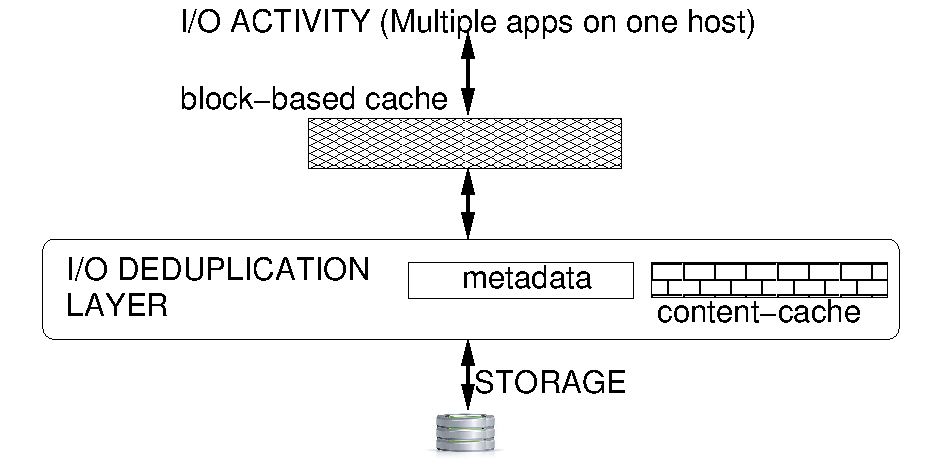
\includegraphics[scale=0.65]{confided-figures/main/sys-arch-iodedup-host.pdf}
\vspace{-0.15in}
\caption{System Architecture of IODEDUP}
\label{fig:iodedup-arch}
%\vspace{-0.2in}
\end{figure}

\subsection{Motivation for in-depth analysis}
Our work is motivated by a few observations from the work
presented in \cite{iodedup}.
First, it demonstrates that a content-addressed cache
is strictly better than a location-addressed cache of the same size. However, since
IODEDUP has both a \textit{block-cache} (i.e., page/buffer cache)
and a \textit{content-cache}, it is
essential to explore the holistic effects of subtracting from the existing
block-cache size while creating the new content-cache.
%For example, 
%within a total cache size of 1 GB, reserving 200MB as a content-addressed
%cache leaves only 800MB as the regular location-addressed cache.
%Fig.~\ref{fig:iodedup-arch}(b) shows some of the various configurations of
%block-cache and content-cache sizes within a total cache size (say 1 GB).
%We create a simulation module to study the effects of using different
%content-cache sizes upon the cache-hits incurred.
Second, since the \textit{content-addressed}\index{Content-cache} cache
basically takes away a finite amount of memory space available
to the buffer/page cache, a study is needed to learn the
optimal content-cache size per workload. This is especially important
because content cache usage/benefits may be application/workload
or request-mix specific.
%understand how the split of cache space should be done between the 
%buffer cache (referred henceforth as \textit{block-cache}) and the 
%\textit{content-cache} so as to achieve maximum benefits, and also to know
%whether such an optimal split is application or workload-specific.
%We study these effects in our work using the traces provided in \cite{iodedup}.
%Third, it is noted in \cite{iodedup} that an integrated sector and content
%cache would be the ideal, but complexity of implementation makes it infeasible.
%In the next section, we present our experiments to
%address the first and second points mentioned above, and later we present 
%the design of our I/O deduplication system called CONFIDE.
%In the next section, we present our experiments to study the performance 
%effects of 
%using different content-cache sizes.
Based on above observations, we claim
that a split-cache approach of sub-dividing available
memory space into location-addressed and content-addressed caches, is inefficient.
More specifically, our claims are the following.
\begin{itemize}
    \item As the evaluation of IODEDUP shows~\cite{iodedup}, a content-addressed cache
        succeeds in improving cache hit ratio for a read-only request
        stream, but does not perform as well with a read/write request stream.
        This was attributed~\cite{iodedup} to the journaling process writing varying
        content to same numbered sectors repeatedly.
        %Thus, block-cache is also needed
        %and it is not desirable to increase the size of content-cache
        %too much.
    \item The split-cache approach has a sweetspot-finding dilemma, wherein
        the content-cache needs to be correctly-sized to allow better cache
        utilization.
        %Finding the sweetspot is an exercise in itself, and
        %would be workload dependent.
%   \item This points to the necessity
%       for an I/O deduplication solution that can perform effectively 
%       even with write-intensive workloads.
\end{itemize}

\subsection{Simulation setup and workloads}
To support our claims, we built a custom simulator\index{Simulator} 
(refer Appendix chapter \ref{chap:thesis-simreplay} for 
simulator details) with prototype implementations of the Vanilla and 
IODEDUP~\cite{iodedup} systems.
%that uses a fixed-size
%location-addressed page/buffer cache, and of the I/O Deduplication
%system.
% that reserves part of the buffer cache above as a content-addressed
%cache. 
%As usual, t
The block-cache\index{Block-cache} is looked up 
based on block numbers as usual, whereas
the content-cache can be looked up based on both block number
and content.
IODEDUP maintains metadata containing MD5~\cite{md5}
hashes of content, to identify similarity.

A high-level overview of the working of Vanilla and IODEDUP~\cite{iodedup}
systems is as follows.
In Vanilla system, a read request's block number is first looked up
into block-cache. Upon hit, content is served whereas upon miss,
the block is fetched from disk. In I/O Deduplication system, the
original disk fetch path due to block-cache miss, is
intercepted and metadata is used to lookup the block in
the content-addressed cache.
Upon a hit in content-cache, the content is returned straight-away to callee
and thus, the disk fetch is \textit{averted}.
However, upon a content-cache miss, a
disk fetch becomes inevitable, and the fetched content is finger-printed
by a hash function like MD5 and metadata is updated.
For our exploration of IODEDUP system's effectiveness,
we chose six content-cache size settings as 10\%,
20\%, 30\%, 50\%, 70\% and 90\% of the total memory size, and
remaining as the size of block-cache. We replay each trace
with a total memory size of 1 GB or 512 MB, as specified in each
experiment respectively.

Evaluation in~\cite{iodedup} is performed with 
traces\index{Workload traces} over 21 days from three production systems
%that were in active use 
at FIU Computer Science Department:
(i)~\textit{webvm}, traces from two virtualized web-servers hosting webmail
proxy and course management system, (ii)~\textit{mail}, traces from an
email server, and (iii)~\textit{homes}, traces from a file server.
From the above,
we consider the entire available \textit{webvm}
and \textit{homes} trace, and one day's trace for \textit{mail} workload,
for our evaluation.

\begin{figure}[t]
    \subfloat[]{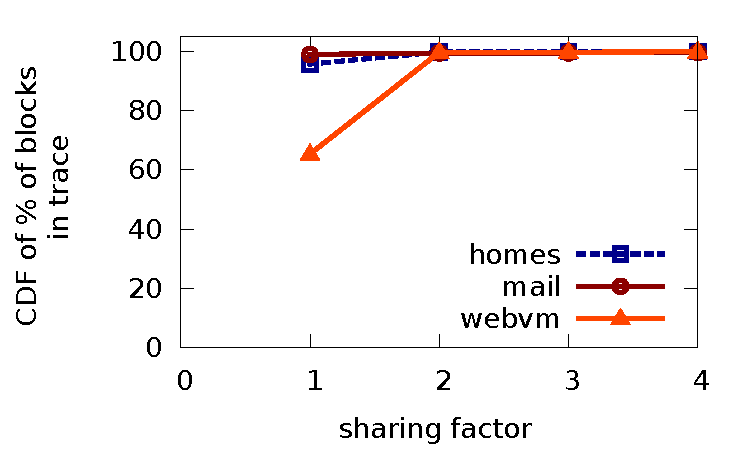
\includegraphics[scale=0.6]{confided-figures/sharing-distrib-from-hashes/reads-writes/cdf-perc-sharing-distrib.pdf}}	\hfill
    \subfloat[]{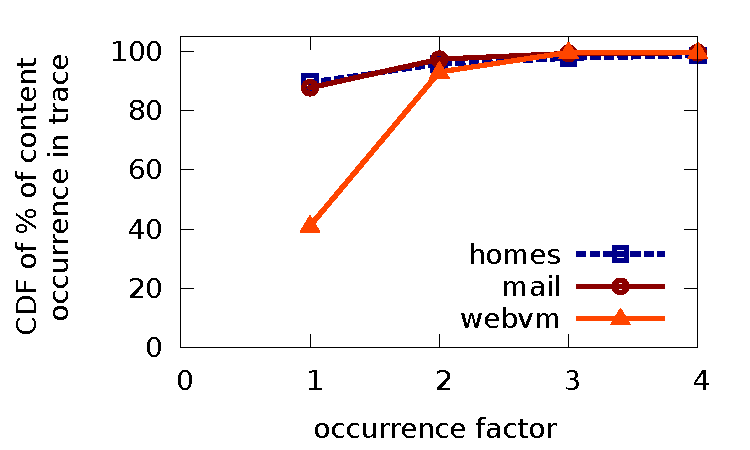
\includegraphics[scale=0.6]{confided-figures/occurrence-distrib/reads-writes/cdf-perc-occurrence-distrib.pdf}} \\
	\null\hfill
\subfloat[]{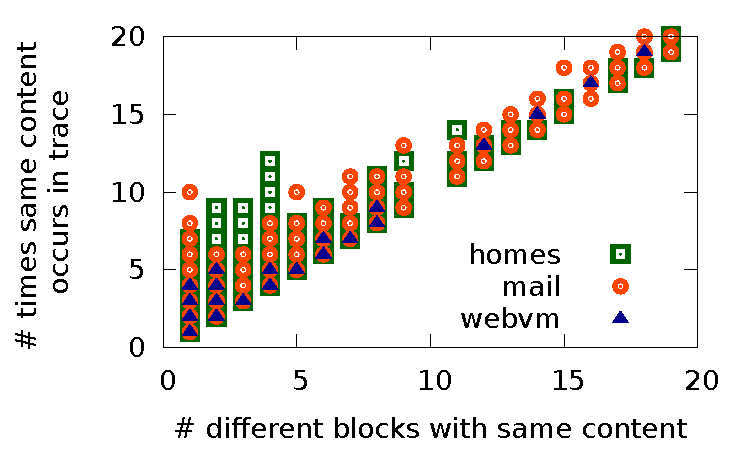
\includegraphics[scale=0.6]{confided-figures/degree-sharing-vs-num-occur-from-hashes/reads-writes/deg-sharing-vs-num-occur.pdf}}
	\hfill\null
    \caption{Study of content similarity in \textit{webvm}, \textit{homes} and \textit{mail} trace workloads.} %online at \cite{iodedup-online}}
\vspace{-0.1in}
\label{fig:similarity-distrib}
\end{figure}

\begin{table}
%\vspace{0.1in}
\centering
\caption{Summary statistics of traces used for evaluation}
%\noindent\makebox[\textwidth]{% 
\begin{tabular}{|l|c|c|c|c|c|} \hline
\textbf{Trace} & \textbf{Num of} & \textbf{Num of} & \textbf{Max} & \textbf{Max} & \textbf{Write} \\
\textbf{Name} & \textbf{read} & \textbf{write} & \textbf{sharing} & \textbf{occurrence} & \textbf{intensivity} \\
\textbf{} & \textbf{requests} & \textbf{requests} & \textbf{factor} & \textbf{factor} & \textbf{factor}  \\ \hline
\textit{homes} & 4,052,176 & 17,110,222 & 5904 & 5905 & 4.2 \\ \hline
\textit{mail} & 2,375,409 & 18,007,471 & 57015 & 57015 & 7.6 \\ \hline
\textit{webvm} & 3,116,456 & 11,177,702 & 124 & 125 & 3.6 \\ \hline
\end{tabular}
%}
%\vspace{-0.3in}
\label{tab:stat-summary}
\end{table}

\subsection{Study of similarity in workloads under consideration}
\label{sec:similarity-study}

To study the content similarity in the workloads under consideration,
we identify the two factors that contribute to the similarity: 
(i) content similarity in the data on disk (irrespective of workload), 
and (ii) access pattern of these similar blocks in the workload.
Basically, even if all blocks on disk have duplicates, the I/O workload
may still not have any duplicates if the access is such that identical
content blocks are never accessed in the same workload. On the other
hand, even if only a small percentage (say 10\%) of blocks have duplicates, 
the I/O workload can still have a high deduplication potential if
most of the blocks being accessed in the workload are from this
small set of duplicated blocks. To distinguish these two factors,
we define the following:-

\begin{enumerate}
\item \textit{Sharing factor} refers to different
blocks (i.e. block addresses) ``sharing'' identical content\index{Content similarity}.
\item \textit{Occurrence factor} refers to occurrences of identical content
in the workload, % (due to same or different blocks),
where ``occurrence'' of identical content can be due to the
same block or due to different blocks having identical content. 
\end{enumerate}

Since we do not have access to the actual underlying data for these traces, 
the block addresses present in the traces are our only clue to the content similarity 
present in the dataset. Thus, we compute \textit{sharing factor} as an approximation 
of the static content similarity in the data. 
Further, although presence of static content similarity is necessary for I/O 
deduplication efforts to be useful, it is not a sufficient condition. This is 
because no I/O deduplication can occur if those identical blocks are not actually 
accessed by any workloads. Thus, we compute \textit{occurrence factor} as an indicator 
of identical content access in the workloads.
The difference between sharing factor and occurrence factor is that, 
when a single block address occurs multiple times in the trace, it is counted as 
only one when computing the ``sharing'' factor of that block’s content whereas 
every occurrence contributes to the ``occurrence'' factor of that content. 


Fig.~\ref{fig:similarity-distrib}(a) plots a CDF of the percentage of \textit{sharing}.
We can see that in \textit{homes} and
\textit{mail} traces, more than 95\% content is present in only one block, whereas
in \textit{webvm} trace, around 35\% content is present in two blocks.
Fig.~\ref{fig:similarity-distrib}(b) plots a CDF of the percentage of \textit{occurrence}.
It is observed that,
in \textit{webvm} workload, 45\% content occur twice,
whereas \textit{homes} and \textit{mail} workloads have only 6-10\% content
occurring twice.

In Fig.~\ref{fig:similarity-distrib}(c), we present a scatter-plot depicting
the sharing factor versus occurrence factor, for every observed block of content.
In other words, for every observed block of content, 
what is its sharing factor\index{Sharing factor} (plotted on x-axis), 
versus its various number of occurrences\index{Occurrence factor} (plotted on y-axis).
Thus, each point in the scatter-plot represents one or more chunks of unique
content with sharing factor as depicted on x-axis and corresponding
number of occurrences on y-axis. For example, in Fig.~\ref{fig:similarity-distrib}(c),
the triangle appearing with value of x=2 and y=5 implies that in the 
\textit{webvm} trace, there are one or more pieces of content having
sharing factor of 2 and occurrence factor of 5. This alludes to the possibility
that for each such piece of content, both the blocks containing it 
were accessed multiple times in the workload---thus
indicating a significant overall potential for I/O deduplication.

Although the x-axis in
%these graphs 
Fig.~\ref{fig:similarity-distrib}(a) and \ref{fig:similarity-distrib}(b)
is cropped to
value of 4, the maximum sharing and occurrence factors
are much higher, and are listed in Table \ref{tab:stat-summary}.
The table presents an overall summary of the traces,
listing number of read and write requests, and
maximum \textit{sharing}, \textit{occurrence} and
\textit{write-intensivity} factors of each trace.
We define \textit{write-intensivity}
factor as the ratio of number of blocks written to number of blocks read. Since
we perform read I/O redirection\index{I/O redirection} 
and do not optimize writes, this factor
will impact effectiveness of cache, as explored later.
\\
\\
The above study indicates that \textit{webvm} workload is a better candidate to
benefit from I/O redirection \& deduplication techniques. However,
%the other two traces
%also have small amounts of duplication, and hence 
we use all three workloads
to perform our experiments. We wish to demonstrate that if a workload has
``any'' significant level of duplication, I/O deduplication can be beneficial
\textit{if and only if} performed effectively. By this, we intend to emphasize
that I/O deduplication is best suited for read-only workloads and its benefits 
keep proportionately decreasing/changing with ratio of read-write requests 
in workloads. Thus, benefits of IODEDUP approach can be less under realistic 
workloads like read-write workload and under practical conditions where a 
block cache is irreplaceable/unavoidable. In such realistic scenarios, we 
claim that our algorithm works far better as demonstrated in following sections.

\begin{figure}
	\begin{minipage}{0.9\textwidth}
\vspace{-1in}
\hspace{-1.5in}
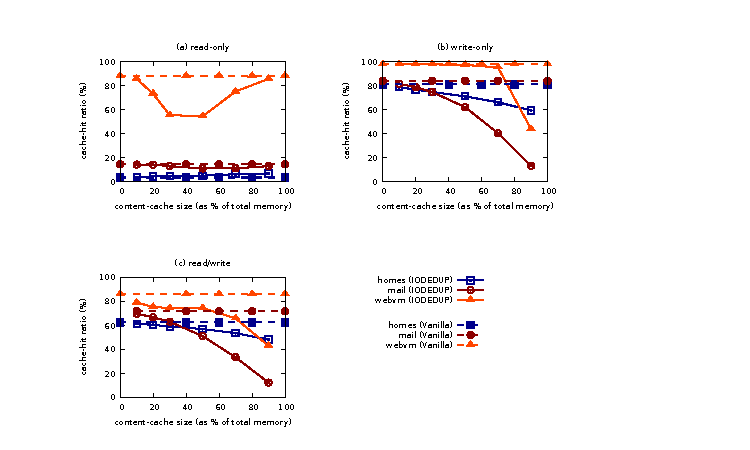
\includegraphics[scale=1.95]{drivechap-figures/sweetspot/sweetspot-multiplot-revised.pdf}
	\vspace{-0.5in}
	\caption{Cache-hit ratios for IODEDUP upon \textit{webvm}, \textit{homes} and \textit{mail} workloads. The total cache size is 1 GB.}
%, and content-cache size as the specified \% of the total.}
\label{fig:sweetspot}
% \vspace{-0.25in}
	\end{minipage}
\end{figure}



\subsection{Comparison of cache-hit ratios}

Fig.~\ref{fig:sweetspot}(a) shows the cache hit ratio for read-only
request traces.
For the \textit{homes} and \textit{mail} workload,
at all settings of content-cache size,
IODEDUP has higher cache-hit ratio than Vanilla. Also, the cache-hit
ratio increases as the \% of content-cache size increases.
However, for the \textit{webvm} trace,
IODEDUP performs worse than Vanilla at all settings. This
is concluded to be because
1 GB total cache size is
already sufficient enough for Vanilla system to cache all relevant
blocks, hence achieving a high cache-hit ratio of almost 90\%.
%Also note that, the number of cache hits does not follow a monotonously 
%increasing or decreasing function.
%This effect is caused due to the interplay of the following
%factors: (i)~the amount of duplicate content in different locations, 
%(ii)~the degree of duplicate content in unique locations accessed, and
%(iii)~the size of the reserved content-addressed cache within total space.
%For example, when block-cache already achieves a high cache-hit ratio, 
%an extra content-cache may be unable to add any extra 
%value and instead the duplication of blocks between the block-cache and
%content-cache only results in wasted space. 

Fig.~\ref{fig:sweetspot}(b) shows the cache hit ratio for write-only
request traces. Disk accesses with Vanilla block-cache has
a higher number of cache hits than IODEDUP\index{IODEDUP} split-cache. 
This is due to varying content being written repeatedly to the same
locations by journalling processes.
For example, non-identical content written to the same block location
intermittently,
results in cache-hit in the vanilla block-cache (due to block number match)
but causes cache-miss in the IODEDUP content-cache (due to content mismatch).
This is also the reason why,
as the content-cache size increases and block-cache size decreases, the
cache hit ratio for write request streams decreases. This is true for
all three workloads considered, and the sweetspot for highest cache-hit
ratios can be considered to be at 100 MB for all three.



Fig.~\ref{fig:sweetspot}(c) shows the cache hit ratios
for traces considering both reads and writes. As can be seen,
the read-only and write-only curves seem to merge in an additive fashion
to form the curves for the read/write traces for all three workloads.
For example, in spite of very low cache-hit ratio in the read-only case,
the \textit{homes} and \textit{mail} workloads have significantly improved
cache-hit ratios in the read/write replay. This is attributed to the
higher number of cache-hits incurred by the write requests (as seen in
Fig.~\ref{fig:sweetspot}(b)).
%On the contrary, the \textit{webvm} 
%workload performed very well for both read-only and write-only
%traces, but shows a slight drop in cache-hit ratios for the read/write 
%trace.

From above experiments, we see that for each request-mix type, IODEDUP has a
different optimal setting for content-cache size---
90\% (900MB) for read-only,
10\% (100 MB) for write-only, and
10\% (100 MB) for read/write.
These settings result in the highest cache hit
ratios for the three workloads using IODEDUP system. Since real
workloads would be read/write workloads, we consider 10\% (100 MB) as
the sweetspot setting for the rest of the evaluation in this thesis.

\subsection{Comparison of number of disk reads averted}
Next, let us take
a look at the metric of ``disk reads averted'', i.e., disk reads avoided owing
to cache hits. 
The difference between the two metrics of \textit{cache hit
ratio}\index{Cache hit ratio} and 
\textit{disk reads averted}\index{Disk reads averted} 
is that even though the cache
experiences churn due to both read and write requests, the former metric
captures all cache-hits whereas the latter captures the cache-hits
occuring on account of read requests only.
%Trivially, both metrics 
%are equivalent for a read-only trace, and a write-only trace contains no 
%read requests needing aversion. Thus, we study this metric especially
%for the trace replay of both reads and writes.

\begin{figure}
    \centering
    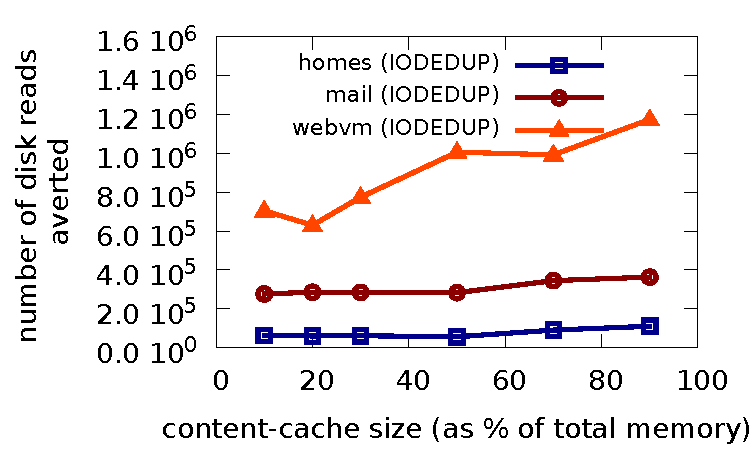
\includegraphics[scale=0.65]{confided-figures/sweetspot/reads-writes/sweetspotaverted-reads-n-writes.pdf}
\caption{Disk reads averted for IODEDUP upon \textit{webvm}, \textit{homes} and \textit{mail} workloads. The total cache size used is 1 GB.}
\label{fig:sweetspot-averted}
%\vspace{-.2in}
\end{figure}

Fig.~\ref{fig:sweetspot-averted} shows the number of disk reads averted
in each of the traces in presence of both reads and writes.
In all three workloads, when content-cache size increases from 10\% to
90\% of the total size, the number of disk reads averted almost doubles
for all three workloads.
%If we judge the number of disk reads averted as 
%a measure of performance since our aim is only read I/O deduplication, 
Judging by ``number of disk reads averted'' as a measure of performance,
a setting of 90\% for content-cache size seems to be the sweetspot
for all three read/write traces. However, this is contrary to our earlier
conclusion that 10\% is the sweetspot setting, which had been based
on ``cache-hit ratio'' as a measure of performance.

The above discrepancy can be explained as follows. When the same block
is written repeatedly with varying content, they all count as cache misses
in content-cache though they will be counted as cache hits if that
block is present in sector-cache too. Thus, in presence of write
requests, total cache hits would be higher when the sector-cache is big
at 90\%, i.e. content-cache is small like 10\%. However, when we
consider the metric of ``disk reads averted'', we see that more number
of disk reads are averted when the content cache size is
bigger, i.e. a content cache size of 90\% results in highest deduplication
for disk read requests although many of the write requests result in cache 
misses due to the smaller (size 10\%) location-addressed cache.

Thus, when we consider the metric of ``disk reads averted'' (which is
basically what I/O deduplication is intended to achieve), we see that
more number of disk reads are averted when the content cache size is
bigger, i.e. a content cache size of 90\% results in highest deduplication.
In other words, when read/write traces are considered, simply sizing the
content cache to improve the overall cache hit ratio does not guarantee the
highest achievable deduplication---this is a major drawback of the
I/O deduplication implementation of~\cite{iodedup}.


\subsection{Effect of excess memory pressure}
\begin{figure}
    \centering
    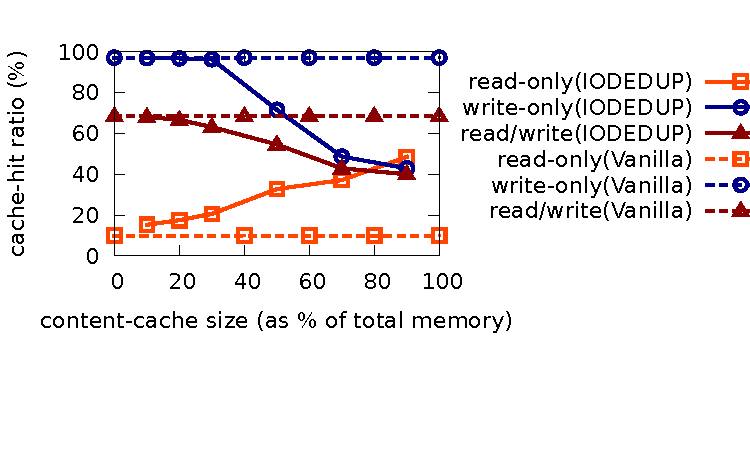
\includegraphics[scale=0.80]{confided-figures/sweetspot-512MB/sweetspot-512MB.pdf}
\vspace{-0.5in}
\caption{Cache-hit ratios for IODEDUP upon \textit{webvm} workload. 
Total cache size 512 MB.}
\vspace{-0.05in}
%, and content-cache size as the specified \% of the total.}
\label{fig:sweetspot-512MB}
\end{figure}

We claimed above that if the total memory
size is already enough to sustain most block requests,
an explicit content-addressed cache does not add much value
and instead degrades the performance (refer
\textit{webvm} workload in Fig.~\ref{fig:sweetspot}(a)).
To substantiate this claim, we performed trace replay for \textit{webvm}
workload with a total memory size setting of only 512 MB. The cache-hit
ratios for read-only, write-only
and read/write replays are illustrated in Fig.~\ref{fig:sweetspot-512MB}.
We can see that the read-only trace exhibits
lowest performance at a content-cache setting of 10\% and the highest
at 90\%. However, the performance of write-only trace and read/write trace
varies inversely as compared to read-only trace, achieving the lowest
performance at a content-cache setting of 90\% and the highest
at 10\%.
Since Vanilla does not perform as well here as with the 1 GB
setting, IODEDUP succeeds in improving the performance by
almost 4$\times$ for the read-only trace
at a content-cache setting of 90\%. However, note that performance of
IODEDUP for both write-only and read/write traces still remain below par,
up to 55\% and 42\% worse than Vanilla, respectively.
\\
\\
The above analysis shows that the dual metrics of \textit{cache-hit
ratios} and \textit{disk reads averted} have different behaviour in relation to the
content-cache sizing of IODEDUP system. Specifically,
for a total memory size of 1 GB,
highest cache-hit
ratios are achieved at a setting of 10\% (refer Fig.~\ref{fig:sweetspot})
and highest number of disk reads
are averted at a setting of 90\% (refer Fig.~\ref{fig:sweetspot-averted}).
Moreover,
the split-cache approach of IODEDUP results in duplicate content across the
block-cache and content-cache, hence degrading the overall performance
(refer Fig.~\ref{fig:sweetspot}).
We conclude that the split-cache approach is inefficient, 
and establish the necessity
%especially in presence of write requests.
%This points to the necessity
for an I/O deduplication solution that can perform effectively
even in presence of write-intensive workloads.

